\chapter{Wild West}

\begin{figure}[!h]
    \centering
    \begin{minipage}[t]{\minipageSize}\centering
      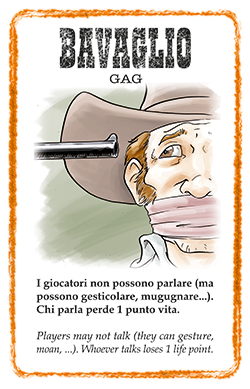
\includegraphics[width=\cardSize\linewidth]{wildwest/06_bavaglio.png}
      \caption[Bavaglio]{Hráči nesmú hovoriť (môžu gestikulovať, stonať, ...). Každý, kto prehovorí, stratí 1 život.}
    \end{minipage}
    \hfill
    \begin{minipage}[t]{\minipageSize}\centering
      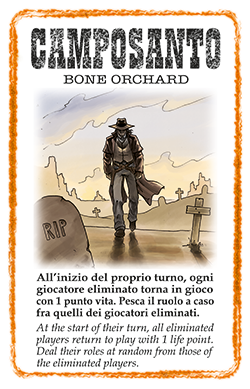
\includegraphics[width=\cardSize\linewidth]{wildwest/06_camposanto.png}
      \caption[Camposanto]{Na začiatku svojho ťahu sa všetci vyradení hráči vrátia do hry s 1 životom. Role vyradených hráčov zamiešajte a náhodne rozdeľte. Hráči sa do hry vracajú stále, aj po skončení efektu, ak sú stále v hre.}
    \end{minipage}
    \hfill
    \begin{minipage}[t]{\minipageSize}\centering
      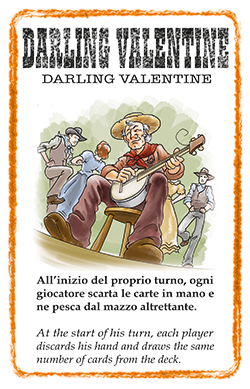
\includegraphics[width=\cardSize\linewidth]{wildwest/06_darlingvalentine.png}
      \caption[Darling Valentine]{Na začiatku svojho ťahu odhodí každý hráč všetky karty z ruky a doberie si rovnaký počet z balíčka. Hráč na ťahu po odhodení a dobratí kariet pokračuje fázou 1.}
    \end{minipage}
    \hfill
    \begin{minipage}[t]{\minipageSize}\centering
      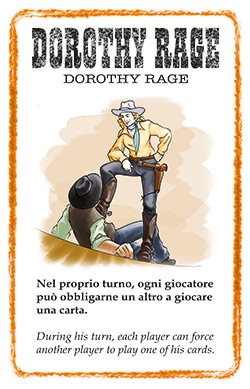
\includegraphics[width=\cardSize\linewidth]{wildwest/06_dorothyrage.png}
      \caption[Dorothy Rage]{Hráč na ťahu môže pomenovať kartu a vybrať hráča, ktorý ju musí zahrať, ak ju má. Musí pritom vopred opísať celú akciu vrátane cieľa. Ak túto kartu hráč nemá, ukáže svoju ruku všetkým hráčom. Ak ju má, zahrá ju v rámci svojich vlastných pravidiel a parametrov, teda podľa svojho dostrelu, svojich schopností a svojich postihov či bonusov. Za všetkých okolností sa ráta, že kartu zahral tento prinútený hráč, nie ten, kto mu to nariadil.}
    \end{minipage}
\end{figure}

\begin{figure}[!h]
    \centering
    \begin{minipage}[t]{\minipageSize}\centering
      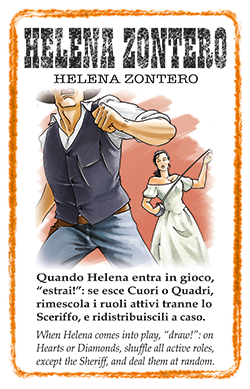
\includegraphics[width=\cardSize\linewidth]{wildwest/06_helenazontero.png}
      \caption[Helena Zontero]{Otočte vrchnú kartu z balíčka: ak sú to srdcia alebo káry, všetky role okrem šerifa sa zamiešajú a náhodne prerozdelia.}
    \end{minipage}
    \hfill
    \begin{minipage}[t]{\minipageSize}\centering
      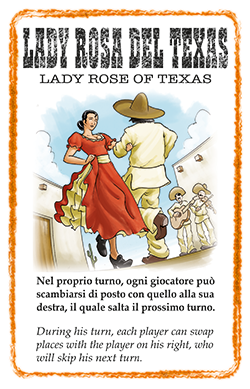
\includegraphics[width=\cardSize\linewidth]{wildwest/06_ladyrosadeltexas.png}
      \caption[Lady Rosa del Texas]{Počas svojho ťahu si môže každý hráč vymeniť miesto s hráčom po svojej pravici, ktorý preskočí svoj najbližší ťah. Hráči si prenesú svoje karty, postavy, role aj životy. Aby sa zabránilo nekonečným slučkám, odporúča sa obmedziť počet bezprostredne po sebe idúcich použití tohto efektu najviac na počet žijúcich hráčov.}
    \end{minipage}
    \hfill
    \begin{minipage}[t]{\minipageSize}\centering
      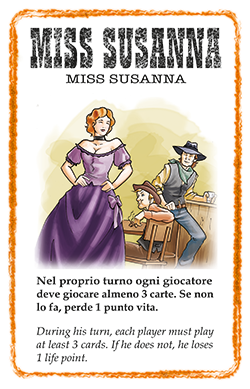
\includegraphics[width=\cardSize\linewidth]{wildwest/06_misssusanna.png}
      \caption[Miss Susanna]{Počas svojho ťahu musí každý hráč zahrať aspoň 3 karty. Kto to neurobí, stratí 1 život. Počítajú sa aj karty zahrané ešte predtým, než Miss Susanna vstúpila do hry v tom istom ťahu. Neplatí pre hráčov, ktorí preskakujú ťah kvôli Väzeniu.}
    \end{minipage}
    \hfill
    \begin{minipage}[t]{\minipageSize}\centering
      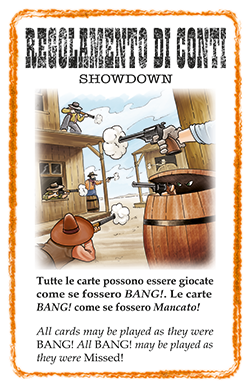
\includegraphics[width=\cardSize\linewidth]{wildwest/06_regolamentodiconti.png}
      \caption[Showdown]{Každú kartu možno hrať ako kartu Bang!. Každá karta Bang! musí byť zahraná ako karta Vedle!. Big Spencer môže použiť kartu Bang! ako kartu Vedle! a Lee Van Kliff môže na aktiváciu svojej schopnosti odhodiť ľubovoľnú z týchto dvoch kariet.}
    \end{minipage}
\end{figure}

\begin{figure}[!h]
    \centering
    \begin{minipage}[t]{\minipageSize}\centering
      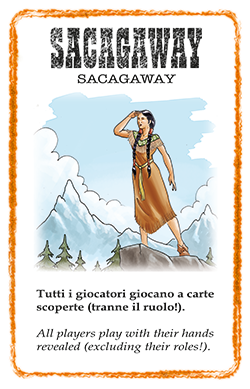
\includegraphics[width=\cardSize\linewidth]{wildwest/06_sacagaway.png}
      \caption[Sacagaway]{Všetci hráči hrajú s odhalenými kartami na ruke, okrem rolí. Ak má dôjsť k náhodnému alebo skrytému odobratiu karty z ruky, napr. pri Panike!, Cat Balou a podobných efektoch, dotknutý hráč svoju ruku dočasne skryje, premieša a karta sa odoberie bez znalosti jej identity. Po odobratí svoju ruku znovu odhalí.\cite{Wildwest}}
    \end{minipage}
    \hfill
    \begin{minipage}[t]{\minipageSize}\centering
      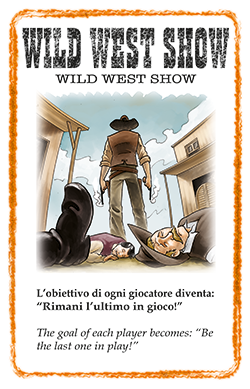
\includegraphics[width=\cardSize\linewidth]{wildwest/06_wildwestshow.png}
      \caption[Wild West Show]{Cieľ každého hráča je: „Zostaň posledný v hre!“. Role ostávajú rovnaké, ale cieľ každého hráča je rovnaký ako pri odpadlíkovi. Schopnosti rolí sa zachovávajú. Šerif nemôže ísť do Väzenia, za zabitie banditu sa stále získava odmena a ak šerif zabije vicešerifa, jeho postih stále platí. Hra pokračuje aj po vyradení šerifa.}
    \end{minipage}
    \hfill
    \begin{minipage}[t]{\minipageSize}\centering
      % \includegraphics[width=\cardSize\linewidth]{}
    \end{minipage}
    \hfill
    \begin{minipage}[t]{\minipageSize}\centering
      % \includegraphics[width=\cardSize\linewidth]{}
    \end{minipage}
\end{figure}
